%!TEX root=../paper.tex

\chapter{Web: A Universal Application Platform}
\label{sec:background}

In this section, I first present the broad scope of the Web computing that this dissertation focuses on (\Sect{sec:background:scope}). I then briefly introduce Web languages and the Web browser runtime (\Sect{sec:background:browser}). Overall, I show that the Web has become a cornerstone technology in today's mobile computing era. Its evolution is largely driven by innovations made in programming languages and system design. These observations motivate my effort on designing a holistic energy-efficient mobile Web computing substrate.

\section{The Scope of the Web}
\label{sec:background:scope}

Web applications are applications developed using Web languages, including HTML, CSS, and JavaScript. Originally, webpages running in a Web browser were the only form of Web application. The scope of the Web today has been greatly expanded beyond webpages to a universal application development platform. The driving force is Web's ``write-once, run-anywhere'' feature that tackles the notorious device fragmentation issue~\cite{fragmentation}. Strategy Analytics reported that by the year 2015 63\% of all business mobile applications are based on Web technologies~\cite{html5rise}.

Mobile system vendors are actively embracing Web technologies. Both iOS and Android provide developers APIs that expose Web browser functionalities~\cite{uiwebview,webview}. This allows developing ``hybrid'' applications that are internally based on Web technologies, but are wrapped by a native shell. Such a development strategy has been widely adopted by popular mobile Apps such as Uber and Instagram~\cite{hybridapp}. In this dissertation, the scope of Web application extends beyond webpages to also include such hybrid applications.

\section{Web Languages and The Web Browser Runtime}
\label{sec:background:browser}

HyperText Markup Language (HTML), Cascading Style Sheets (CSS), and JavaScript are the three fundamental languages for Web development. In a nutshell, HTML describes the structural information of a Web application by building a Document Object Model (DOM) tree~\cite{DOM}, in which each node represents a Web application element. CSS describes an application's style information by declaring visual properties of each DOM tree node. JavaScript specifies an application's dynamic behavior by defining callback functions to execute when certain user interactions are triggered on DOM nodes.

To enable portability of Web applications, the Web browser acts as a ``virtual machine'' or a runtime system layer that dynamically translates HTML, CSS, and JavaScript to different platforms. \Fig{fig:data-flow} shows the overall flow of execution within any typical Web browser, which typically consists of two core modules: a rendering engine (e.g., WebKit for Chrome and Gecko for Firefox) that translates HTML and CSS, and a JavaScript engine that executes JavaScript code.

\begin{figure}[t]
\centering
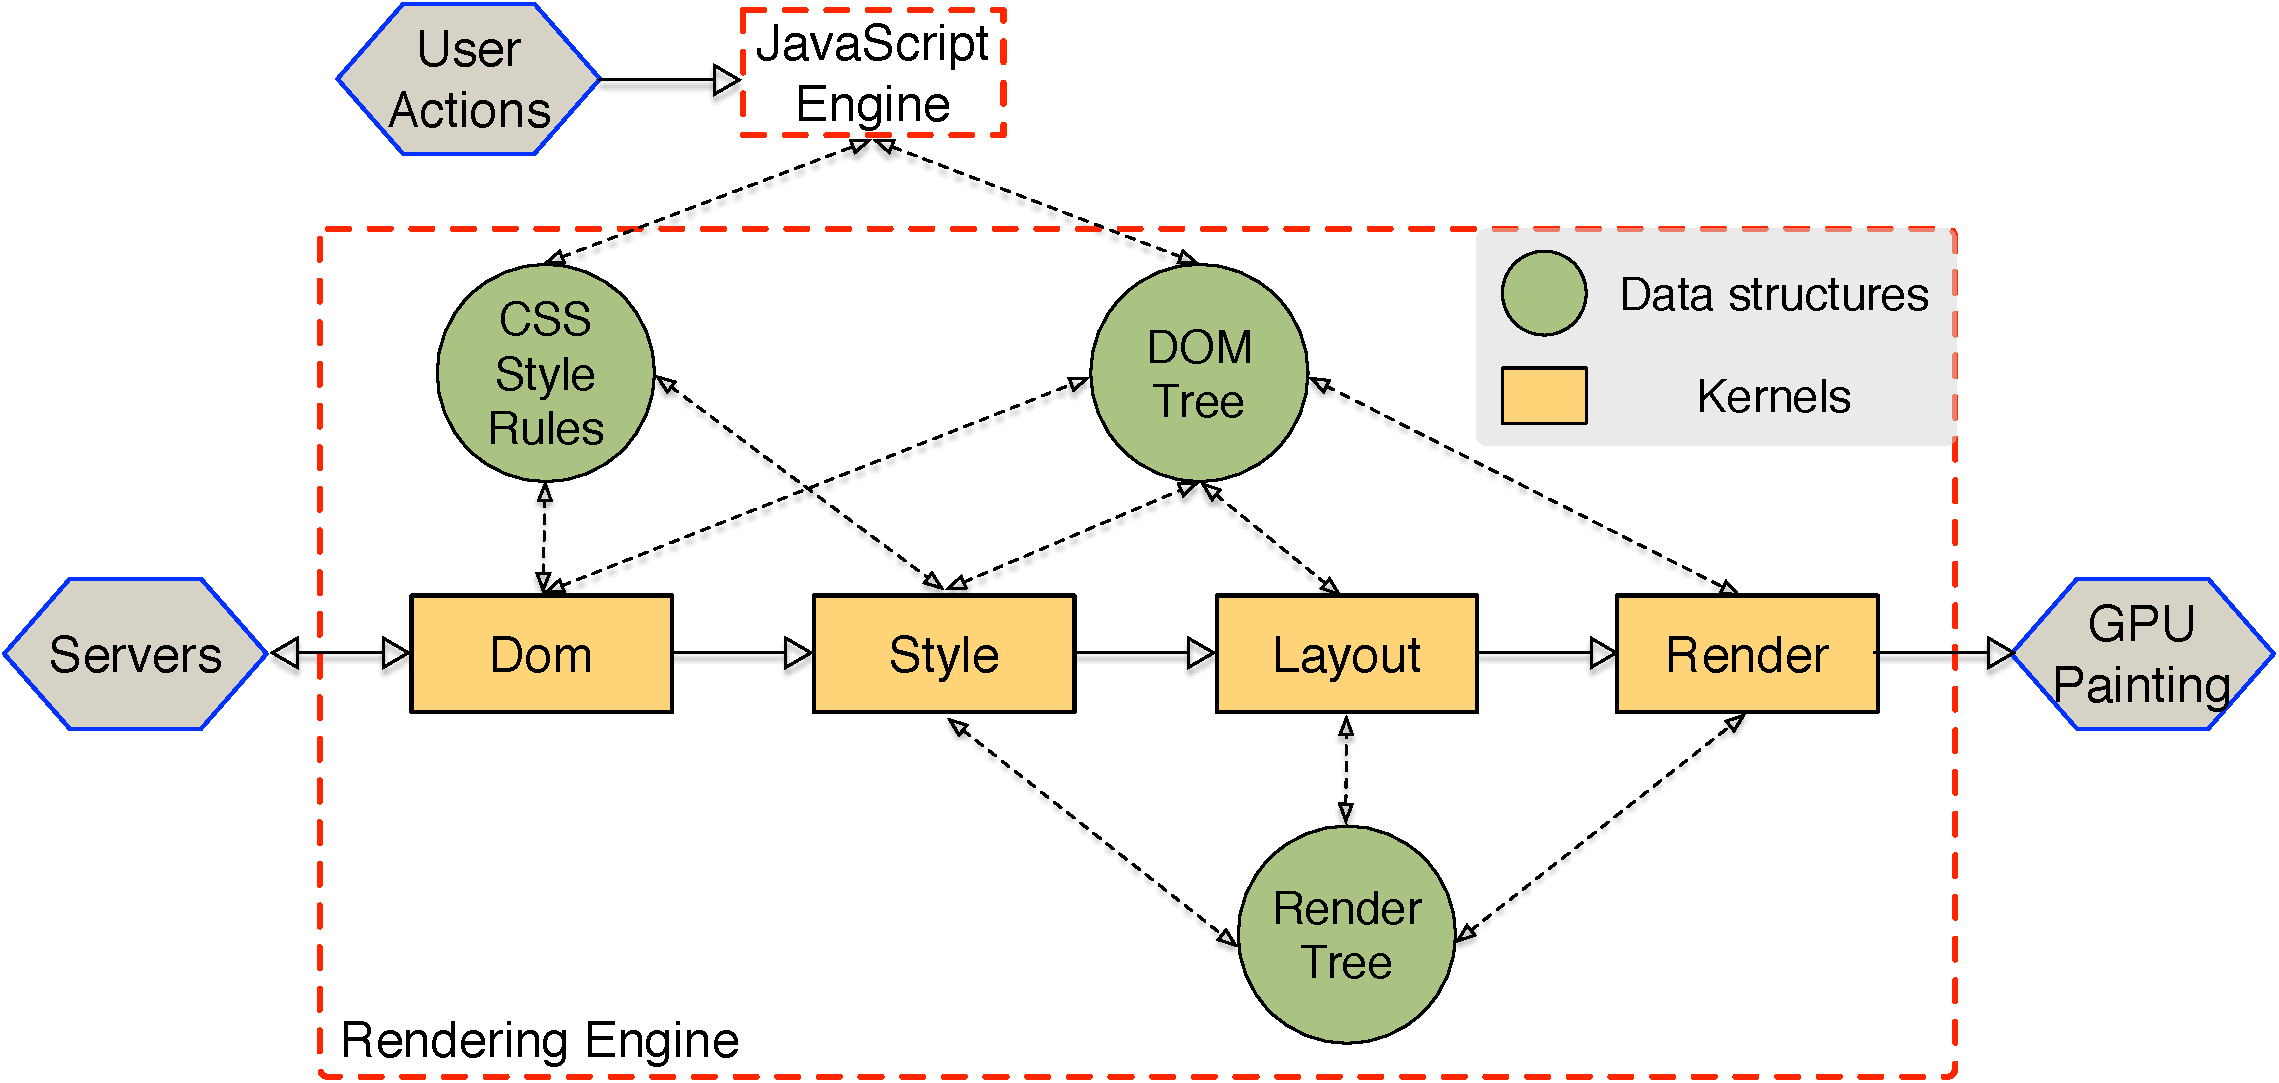
\includegraphics[trim=0 0 0 0, clip, width=\columnwidth]{data-flow}
\caption{A typical Web browser architecture.}
\label{fig:data-flow}
\end{figure}

The rendering engine mainly consists of four kernels:~\textit{Dom}, \textit{Style}, \textit{Layout}, and \textit{Render}. The kernels, shown in boxes, process the webpage and prepare pixels for a GPU to paint. The figure also shows the important data structures that the kernels consume. The DOM tree, CSS style rules, and Render tree are those important data structures, and they are heavily shared across the kernels. The data structures are shown in circles with arrows indicating information flow between the kernels. 

The~\textit{Dom} kernel is in charge of parsing the webpage contents. Specifically, it constructs the DOM tree from the HTML files, and extracts the CSS style rules from the CSS files. Given the DOM tree and CSS style rules, the~\textit{Style} kernel computes the webpage's style information and stores the results in the render tree. Each render tree node corresponds to a visible element in the webpage. Once the style information of each webpage element is calculated, the~\textit{Layout} kernel recursively traverses the render tree to decide each visible element's position information based on each element's size and relative positioning. The final $<x, y>$ coordinates are stored back into the render tree. Eventually, the~\textit{Render} kernel examines the render tree to decide the $z$-ordering of each visible element so that they can be displayed in the correct overlapping order.

Over the past two decades, language evolution and Web runtime design have been constantly driving Web  innovations~\cite{webevolution,html5evolution}. As a result, current Web standards such as HTML5 and CSS3 enable ever-richer functionalities, such as offline storage, media playback, and geolocation, that are the core in today's mobile applications. Web language and browser design innovations will continue to be the key enabler for next-generation Web computing.

